% Options for packages loaded elsewhere
\PassOptionsToPackage{unicode}{hyperref}
\PassOptionsToPackage{hyphens}{url}
\PassOptionsToPackage{dvipsnames,svgnames,x11names}{xcolor}
%
\documentclass[
  french,
]{article}
\title{Econométrie de la finance}
\usepackage{etoolbox}
\makeatletter
\providecommand{\subtitle}[1]{% add subtitle to \maketitle
  \apptocmd{\@title}{\par {\large #1 \par}}{}{}
}
\makeatother
\subtitle{Chapitre 3: Les modèles non liléaires univariés}
\author{Mohamed Essaied Hamrita}
\date{Octobre 2021}

\usepackage{amsmath,amssymb}
\usepackage{lmodern}
\usepackage{iftex}
\ifPDFTeX
  \usepackage[T1]{fontenc}
  \usepackage[utf8]{inputenc}
  \usepackage{textcomp} % provide euro and other symbols
\else % if luatex or xetex
  \usepackage{unicode-math}
  \defaultfontfeatures{Scale=MatchLowercase}
  \defaultfontfeatures[\rmfamily]{Ligatures=TeX,Scale=1}
\fi
% Use upquote if available, for straight quotes in verbatim environments
\IfFileExists{upquote.sty}{\usepackage{upquote}}{}
\IfFileExists{microtype.sty}{% use microtype if available
  \usepackage[]{microtype}
  \UseMicrotypeSet[protrusion]{basicmath} % disable protrusion for tt fonts
}{}
\makeatletter
\@ifundefined{KOMAClassName}{% if non-KOMA class
  \IfFileExists{parskip.sty}{%
    \usepackage{parskip}
  }{% else
    \setlength{\parindent}{0pt}
    \setlength{\parskip}{6pt plus 2pt minus 1pt}}
}{% if KOMA class
  \KOMAoptions{parskip=half}}
\makeatother
\usepackage{xcolor}
\IfFileExists{xurl.sty}{\usepackage{xurl}}{} % add URL line breaks if available
\IfFileExists{bookmark.sty}{\usepackage{bookmark}}{\usepackage{hyperref}}
\hypersetup{
  pdftitle={Econométrie de la finance},
  pdfauthor={Mohamed Essaied Hamrita},
  pdflang={fr},
  colorlinks=true,
  linkcolor={blue},
  filecolor={Maroon},
  citecolor={Blue},
  urlcolor={blue},
  pdfcreator={LaTeX via pandoc}}
\urlstyle{same} % disable monospaced font for URLs
\usepackage[margin=1in]{geometry}
\usepackage{color}
\usepackage{fancyvrb}
\newcommand{\VerbBar}{|}
\newcommand{\VERB}{\Verb[commandchars=\\\{\}]}
\DefineVerbatimEnvironment{Highlighting}{Verbatim}{commandchars=\\\{\}}
% Add ',fontsize=\small' for more characters per line
\usepackage{framed}
\definecolor{shadecolor}{RGB}{248,248,248}
\newenvironment{Shaded}{\begin{snugshade}}{\end{snugshade}}
\newcommand{\AlertTok}[1]{\textcolor[rgb]{0.94,0.16,0.16}{#1}}
\newcommand{\AnnotationTok}[1]{\textcolor[rgb]{0.56,0.35,0.01}{\textbf{\textit{#1}}}}
\newcommand{\AttributeTok}[1]{\textcolor[rgb]{0.77,0.63,0.00}{#1}}
\newcommand{\BaseNTok}[1]{\textcolor[rgb]{0.00,0.00,0.81}{#1}}
\newcommand{\BuiltInTok}[1]{#1}
\newcommand{\CharTok}[1]{\textcolor[rgb]{0.31,0.60,0.02}{#1}}
\newcommand{\CommentTok}[1]{\textcolor[rgb]{0.56,0.35,0.01}{\textit{#1}}}
\newcommand{\CommentVarTok}[1]{\textcolor[rgb]{0.56,0.35,0.01}{\textbf{\textit{#1}}}}
\newcommand{\ConstantTok}[1]{\textcolor[rgb]{0.00,0.00,0.00}{#1}}
\newcommand{\ControlFlowTok}[1]{\textcolor[rgb]{0.13,0.29,0.53}{\textbf{#1}}}
\newcommand{\DataTypeTok}[1]{\textcolor[rgb]{0.13,0.29,0.53}{#1}}
\newcommand{\DecValTok}[1]{\textcolor[rgb]{0.00,0.00,0.81}{#1}}
\newcommand{\DocumentationTok}[1]{\textcolor[rgb]{0.56,0.35,0.01}{\textbf{\textit{#1}}}}
\newcommand{\ErrorTok}[1]{\textcolor[rgb]{0.64,0.00,0.00}{\textbf{#1}}}
\newcommand{\ExtensionTok}[1]{#1}
\newcommand{\FloatTok}[1]{\textcolor[rgb]{0.00,0.00,0.81}{#1}}
\newcommand{\FunctionTok}[1]{\textcolor[rgb]{0.00,0.00,0.00}{#1}}
\newcommand{\ImportTok}[1]{#1}
\newcommand{\InformationTok}[1]{\textcolor[rgb]{0.56,0.35,0.01}{\textbf{\textit{#1}}}}
\newcommand{\KeywordTok}[1]{\textcolor[rgb]{0.13,0.29,0.53}{\textbf{#1}}}
\newcommand{\NormalTok}[1]{#1}
\newcommand{\OperatorTok}[1]{\textcolor[rgb]{0.81,0.36,0.00}{\textbf{#1}}}
\newcommand{\OtherTok}[1]{\textcolor[rgb]{0.56,0.35,0.01}{#1}}
\newcommand{\PreprocessorTok}[1]{\textcolor[rgb]{0.56,0.35,0.01}{\textit{#1}}}
\newcommand{\RegionMarkerTok}[1]{#1}
\newcommand{\SpecialCharTok}[1]{\textcolor[rgb]{0.00,0.00,0.00}{#1}}
\newcommand{\SpecialStringTok}[1]{\textcolor[rgb]{0.31,0.60,0.02}{#1}}
\newcommand{\StringTok}[1]{\textcolor[rgb]{0.31,0.60,0.02}{#1}}
\newcommand{\VariableTok}[1]{\textcolor[rgb]{0.00,0.00,0.00}{#1}}
\newcommand{\VerbatimStringTok}[1]{\textcolor[rgb]{0.31,0.60,0.02}{#1}}
\newcommand{\WarningTok}[1]{\textcolor[rgb]{0.56,0.35,0.01}{\textbf{\textit{#1}}}}
\usepackage{graphicx}
\makeatletter
\def\maxwidth{\ifdim\Gin@nat@width>\linewidth\linewidth\else\Gin@nat@width\fi}
\def\maxheight{\ifdim\Gin@nat@height>\textheight\textheight\else\Gin@nat@height\fi}
\makeatother
% Scale images if necessary, so that they will not overflow the page
% margins by default, and it is still possible to overwrite the defaults
% using explicit options in \includegraphics[width, height, ...]{}
\setkeys{Gin}{width=\maxwidth,height=\maxheight,keepaspectratio}
% Set default figure placement to htbp
\makeatletter
\def\fps@figure{htbp}
\makeatother
\setlength{\emergencystretch}{3em} % prevent overfull lines
\providecommand{\tightlist}{%
  \setlength{\itemsep}{0pt}\setlength{\parskip}{0pt}}
\setcounter{secnumdepth}{-\maxdimen} % remove section numbering
\newlength{\cslhangindent}
\setlength{\cslhangindent}{1.5em}
\newlength{\csllabelwidth}
\setlength{\csllabelwidth}{3em}
\newlength{\cslentryspacingunit} % times entry-spacing
\setlength{\cslentryspacingunit}{\parskip}
\newenvironment{CSLReferences}[2] % #1 hanging-ident, #2 entry spacing
 {% don't indent paragraphs
  \setlength{\parindent}{0pt}
  % turn on hanging indent if param 1 is 1
  \ifodd #1
  \let\oldpar\par
  \def\par{\hangindent=\cslhangindent\oldpar}
  \fi
  % set entry spacing
  \setlength{\parskip}{#2\cslentryspacingunit}
 }%
 {}
\usepackage{calc}
\newcommand{\CSLBlock}[1]{#1\hfill\break}
\newcommand{\CSLLeftMargin}[1]{\parbox[t]{\csllabelwidth}{#1}}
\newcommand{\CSLRightInline}[1]{\parbox[t]{\linewidth - \csllabelwidth}{#1}\break}
\newcommand{\CSLIndent}[1]{\hspace{\cslhangindent}#1}
\usepackage[utf8]{inputenc}
\usepackage[french]{babel}
\usepackage[margin=1in]{geometry}
%\usepackage[colorlinks]{hyperref}
\usepackage{natbib}
\usepackage{hyperref}
 \hypersetup{
     colorlinks=true,
     linkcolor=blue,
     filecolor=blue,
     citecolor = blue,      
     urlcolor=blue,
     }
\ifXeTeX
  % Load polyglossia as late as possible: uses bidi with RTL langages (e.g. Hebrew, Arabic)
  \usepackage{polyglossia}
  \setmainlanguage[]{french}
\else
  \usepackage[main=french]{babel}
% get rid of language-specific shorthands (see #6817):
\let\LanguageShortHands\languageshorthands
\def\languageshorthands#1{}
\fi
\ifLuaTeX
  \usepackage{selnolig}  % disable illegal ligatures
\fi

\begin{document}
\maketitle

\hypertarget{introduction}{%
\subsection{Introduction}\label{introduction}}

\begin{itemize}
\item
  Dans ce chapitre nous introduisons quelques modèles non linéaires
  univariés et nous discutons leurs propriétes statistiques.
\item
  Les modèles introduits sont: le modèle TAR (Threshold AR), le modèle
  Markov switching (MSM), smooth threshold autoregressive (STAR) models,
  et time-varying parameter models (TVM)
\end{itemize}

\hypertarget{le-moduxe8le-tar}{%
\subsection{Le modèle TAR}\label{le-moduxe8le-tar}}

\begin{itemize}
\item
  Le modèle TAR est proposé par (\protect\hyperlink{ref-tong78}{Tong
  1978}) et largement utilisé depuis la publication de l'article de
  (\protect\hyperlink{ref-tong80}{Tong et Lim 1980}).
\item
  Nous commençons par un modèle TAR simple à deux régimes, puis nous
  discutons le modèle TAR à régimes multiples.
\item
  \textbf{Définition:} Une série temporelle \(\{X_t\}\) suit un modèle
  TAR d'ordre \(p\) avec la variable seuil \(X_{t-d}\), s'il vérifie la
  relation suivante: \[
  X_t=\begin{cases}
  \phi_0+\displaystyle\sum_{i=1}^p\phi_iX_{t-i}+\sigma_1\varepsilon_t \;,\text{ si }\; X_{t-d} \leq r\\
  \theta_0+\displaystyle\sum_{i=1}^p\theta_iX_{t-i}+\sigma_2\varepsilon_t \;\;,\text{ si }\; X_{t-d} > r
  \end{cases}
  \] avec \(\varepsilon_t \stackrel{iid}{\sim}(0,1)\), \(\phi_i\) et
  \(\theta_i\) des valeurs réelles telles que \(\phi_i \neq \theta_i\)
  pour quelques valeurs de \(i\). \(d\) est entier positif et \(r\)
  représente la valeur seuil (threshold).
\end{itemize}

Le modèle TAR à deux régimes peut s'écrire sous la forme suivante: \[
X_t=\phi_0+\displaystyle\sum_{i=1}^p\phi_iX_{t-i}+\sigma_1\varepsilon_t+I(X_{t-d} > r)\left(\beta_0+\displaystyle\sum_{i=1}^p\beta_iX_{t-i}+\gamma\varepsilon_t \right)
\] où \(I(X_{t-d} > r)=1\) si \(X_{t-d} > r\) et \(0\) sinon.
\(\beta_i=\theta_i-\phi_i\) pour \(i=0,1,\ldots,p\) et
\(\gamma=\sigma_2-\sigma_1\)

\textbf{Exemple:} Soit le processus \(\{X_t\}\) définit par: \[
X_t=\begin{cases}
0.2+0.45X_{t-1}+0.2\varepsilon_t \;,\text{ si }\; X_{t-4} \leq -1\\
0.4+0.6X_{t-1}+0.5\varepsilon_t \;\;,\text{ si }\; X_{t-4} > 1
\end{cases}
\]

\begin{Shaded}
\begin{Highlighting}[]
\FunctionTok{library}\NormalTok{(TSA); }
\FunctionTok{set.seed}\NormalTok{(}\DecValTok{12345}\NormalTok{)}
\NormalTok{x}\OtherTok{=}\FunctionTok{tar.sim}\NormalTok{(}\AttributeTok{n=}\DecValTok{500}\NormalTok{,}\AttributeTok{Phi1=}\FunctionTok{c}\NormalTok{(}\FloatTok{0.2}\NormalTok{,}\FloatTok{0.45}\NormalTok{), }\AttributeTok{Phi2=}\FunctionTok{c}\NormalTok{(}\FloatTok{0.4}\NormalTok{,}\FloatTok{0.6}\NormalTok{),}\AttributeTok{p=}\DecValTok{1}\NormalTok{,}
          \AttributeTok{d=}\DecValTok{4}\NormalTok{,}\AttributeTok{sigma1=}\FloatTok{0.2}\NormalTok{,}\AttributeTok{sigma2=}\FloatTok{0.5}\NormalTok{, }\AttributeTok{thd=}\SpecialCharTok{{-}}\DecValTok{1}\NormalTok{)}\SpecialCharTok{$}\NormalTok{y}
\FunctionTok{plot}\NormalTok{(x, }\AttributeTok{type=}\StringTok{"l"}\NormalTok{, }\AttributeTok{col=}\DecValTok{2}\NormalTok{, }\AttributeTok{xlab=}\StringTok{""}\NormalTok{, }\AttributeTok{ylab=}\FunctionTok{expression}\NormalTok{(X[t]))}
\end{Highlighting}
\end{Shaded}

\begin{center}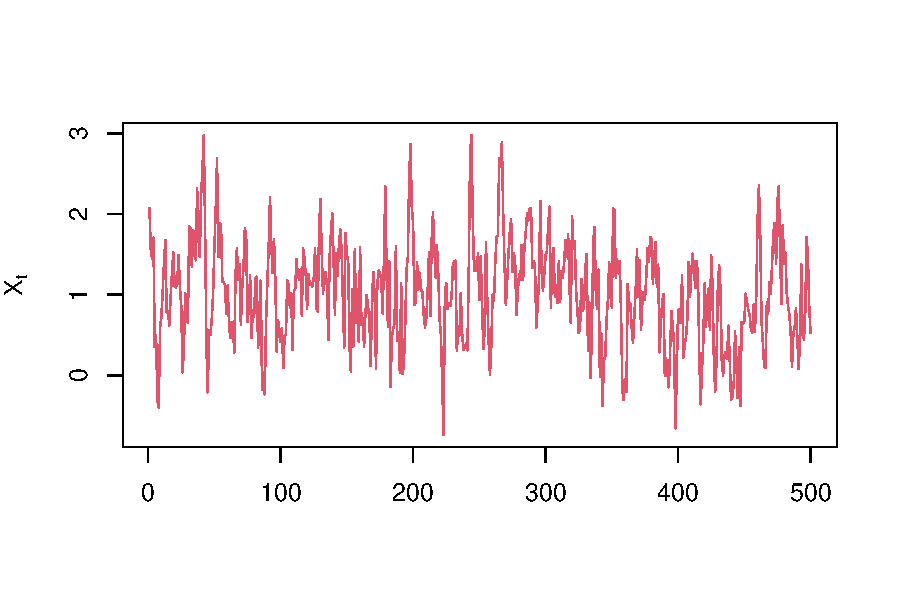
\includegraphics{Chap3_files/figure-latex/tar1-1} \end{center}

\hypertarget{propriuxe9tuxe9s-statistiques}{%
\subsection{Propriétés
statistiques}\label{propriuxe9tuxe9s-statistiques}}

Considérons le modèle TAR\((1)\) à deux régime: \[
X_t=\begin{cases}
\phi_1 X_{t-1}+\sigma_1\varepsilon_t \;,\text{ si }\; X_{t-1} \leq 0\\
\theta_1 X_{t-1}+\sigma_2\varepsilon_t \;\;,\text{ si }\; X_{t-1} > 0
\end{cases}
\] La skeleton de ce modèle est \[
f(X_{t-1})=\begin{cases}
\phi_1 X_{t-1}\;,\text{ si }\; X_{t-1} \leq 0\\
\theta_1 X_{t-1}\;\;,\text{ si }\; X_{t-1} > 0
\end{cases}
\] Puisque \(x_0\) est supposée un réel quelconque, alors pour que la
série \(X_t\) soit stable, il faut que \(\phi_1 < 1\), \(\theta_1 < 1\)
et \(\phi_1 \theta_1 <1\).

Pour \(d>1\), (\protect\hyperlink{ref-chenTsay91}{Chen et Tsay 1991})
ont montré que les conditions de stabilité du modèle est: \(\phi_1 <1\),
\(\theta_1 <1\) et \(\phi_1^{s(d)}\theta_1^{t(d)}\) où \(s(d)=t(d)=1\)
si \(d=1\) et \(s(d)=1\), \(t(d)=2\) si \(d=2\).

\hypertarget{estimation-du-moduxe8le-tar}{%
\subsection{Estimation du modèle
TAR}\label{estimation-du-moduxe8le-tar}}

Le modèle TAR à deux régime peut être estimé soit par la méthode du
maximum de vraisemblance, soit par la méthode des MCO. Ici, on donne la
méthode des MCO. La matrice des variables explicatives peut être écrite
de la forme suivante: \[
X_t(r)=\left(X'_1 \,I(X_{t-d}\leq r)\;\;X'_2\,I(X_{t-d} > r)) \right)
\] d'où, le modèle peut se réécrire comme: \[
X_t=X'_t(r)\alpha+\varepsilon_t\;\text{ où }\; \alpha=(\phi'\;\;\theta')'
\] Pour \(r\) donnée, on obtient: \[
\widehat{\alpha}(r)=\left(X'_t(r)X_t(r)\right)^{-1}X'_t(r)X_t
\]

\textbf{Estimation du paramètre} \(r\): L'estimation du vecteur
\(\alpha\) se fait pour \(r\) fixé. Or, \(r\) est généralement inconnu.
Donc, ce paramètre sera estimé en faisant varier le paramètre \(r\),
soit une séquence de \(n\) valeurs. Pour chaque valeur de \(r\), on
calcul la somme carré des erreurs du modèle estimé, puis on retient la
valeur du \(r\) qui correspond à la somme des carrés des erreurs la plus
faible.

\textbf{Estimation du paramètre} \(d\): Dans la pratique, le paramètre
\(d\) est inconnu et on doit l'estimer. Ce paramètre sera estimé avec le
vecteur \(\alpha\) en imposant \(d \in \{1,2,\ldots,\overline{d}\}\).

\textbf{Test statistique TAR}:

Une question importante est posée: quand le modèle TAR est
statistiquement significative relativement à un modèle linéaire. Il
s'agit de tester: \(H_0:\; \phi=\theta\). Puisque la valeur du seuil
\(r\) est inconnue, un tel test devient délicat.

Pour plus amples discussions, voir (\protect\hyperlink{ref-chan90}{Chan
1990}) et (\protect\hyperlink{ref-hansen97}{Hansen 1997})

\hypertarget{pruxe9vision}{%
\subsection{Prévision}\label{pruxe9vision}}

Pour \(d \geq 1\) donné, la prévision à une étape est donnée par: \[
X_{T+1}=\begin{cases}
\phi_0+\displaystyle\sum_{i=1}^p\phi_iX_{T+1-i},\quad e_{T+1}=\sigma_1\varepsilon_{T+1},\;\;\text{ si } X_{t-d}\leq r\\
\theta_0+\displaystyle\sum_{i=1}^p\theta_iX_{T+1-i},\quad e_{T+1}=\sigma_2\varepsilon_{T+1},\;\;\text{ si } X_{t-d}> r
\end{cases}
\]

\hypertarget{application}{%
\subsection{Application}\label{application}}

On veut modéliser le prix du Cooper. On considère la série des prix
annuels du Cooper allant de 1800 à 1996
(\protect\hyperlink{ref-hyndman2016}{Hyndman et Yang 2018}). La série
est ajustée après avoir éliminer la tendance. La figure suivante montre
l'évolution des prix et la fonction d'auto-corrélation simple.

\begin{Shaded}
\begin{Highlighting}[]
\NormalTok{cooper}\OtherTok{=}\FunctionTok{scan}\NormalTok{(}\StringTok{"https://raw.githubusercontent.com/Hamrita/TSFin/main/Chap3/copper.txt"}\NormalTok{)}
\FunctionTok{par}\NormalTok{(}\AttributeTok{mfrow=}\FunctionTok{c}\NormalTok{(}\DecValTok{1}\NormalTok{,}\DecValTok{2}\NormalTok{))}
\FunctionTok{plot}\NormalTok{(}\DecValTok{1800}\SpecialCharTok{:}\DecValTok{1996}\NormalTok{,cooper, }\AttributeTok{type=}\StringTok{"l"}\NormalTok{, }\AttributeTok{col=}\DecValTok{2}\NormalTok{, }\AttributeTok{xlab=}\StringTok{""}\NormalTok{, }\AttributeTok{ylab=}\StringTok{""}\NormalTok{)}
\FunctionTok{acf}\NormalTok{(cooper)}
\end{Highlighting}
\end{Shaded}

\begin{center}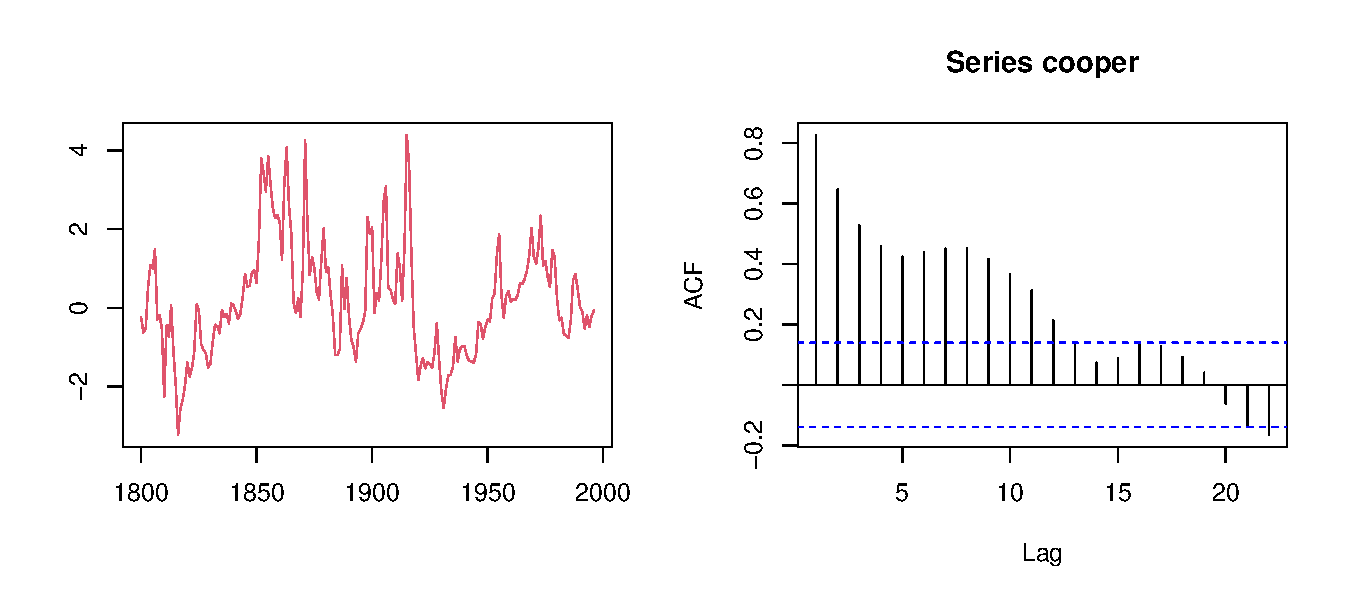
\includegraphics{Chap3_files/figure-latex/unnamed-chunk-2-1} \end{center}

Un premier examen de non linéarité se fait en représentant \(x_t\) en
fonction de \(x_{t-1}\)

\begin{Shaded}
\begin{Highlighting}[]
\NormalTok{y }\OtherTok{\textless{}{-}}\NormalTok{ cooper[}\DecValTok{2}\SpecialCharTok{:}\DecValTok{197}\NormalTok{]; x }\OtherTok{\textless{}{-}}\NormalTok{ cooper[}\DecValTok{1}\SpecialCharTok{:}\DecValTok{196}\NormalTok{]}
\NormalTok{m1 }\OtherTok{\textless{}{-}} \FunctionTok{loess}\NormalTok{(y}\SpecialCharTok{\textasciitilde{}}\NormalTok{x)  }\DocumentationTok{\#\# local smoothing}
\NormalTok{sx }\OtherTok{\textless{}{-}} \FunctionTok{sort}\NormalTok{(x,}\AttributeTok{index=}\NormalTok{T)  }\DocumentationTok{\#\# sorting the threshold variable}
\NormalTok{ix }\OtherTok{\textless{}{-}}\NormalTok{ sx}\SpecialCharTok{$}\NormalTok{ix }\DocumentationTok{\#\# index for order{-}statistics}
 \FunctionTok{plot}\NormalTok{(x,y,}\AttributeTok{xlab=}\StringTok{\textquotesingle{}x(t{-}1)\textquotesingle{}}\NormalTok{,}\AttributeTok{ylab=}\StringTok{\textquotesingle{}x(t)\textquotesingle{}}\NormalTok{)}
\FunctionTok{lines}\NormalTok{(x[ix],m1}\SpecialCharTok{$}\NormalTok{fitted[ix],}\AttributeTok{col=}\StringTok{"red"}\NormalTok{)}
\end{Highlighting}
\end{Shaded}

\begin{center}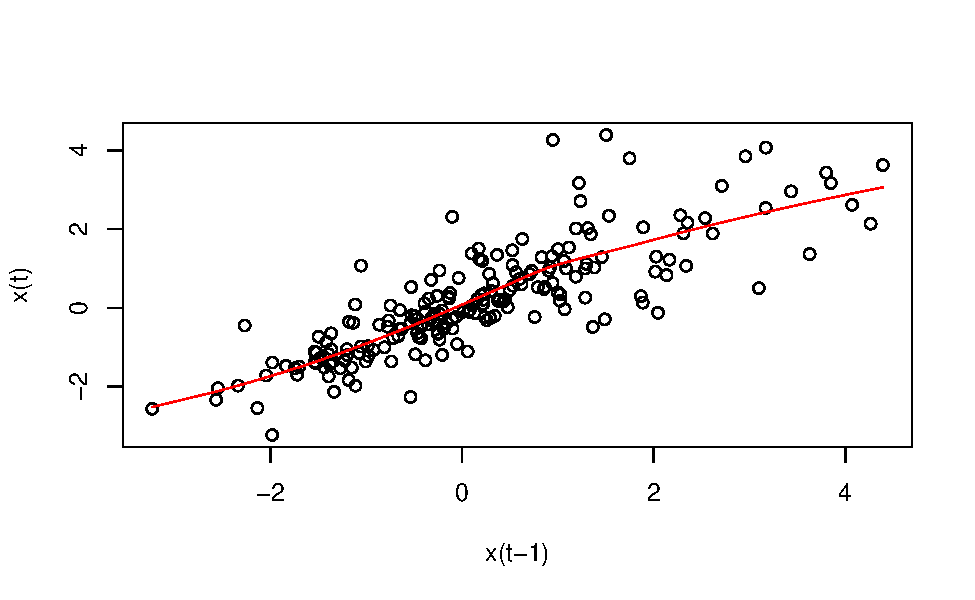
\includegraphics{Chap3_files/figure-latex/unnamed-chunk-3-1} \end{center}

On remarque bien que la dépendance entre \(x_t\) et \(x_{t-1}\) est non
linéaire.

\textbf{Tests de linéarité}

\begin{Shaded}
\begin{Highlighting}[]
\FunctionTok{library}\NormalTok{(nonlinearTseries)}
\NormalTok{tests}\OtherTok{=}\FunctionTok{nonlinearityTest}\NormalTok{(cooper, F)}
\NormalTok{tests}\SpecialCharTok{$}\NormalTok{TarTest}
\end{Highlighting}
\end{Shaded}

\begin{verbatim}
$percentiles
[1] 24.72527 75.27473

$test.statistic
[1] 66.50607

$p.value
[1] 1.896341e-06
\end{verbatim}

On a p-value qui est inférieur à \(5\%\), donc on rejette l'hypothèse
nulle de linéarité du modèle.

\textbf{Estimation}

\begin{Shaded}
\begin{Highlighting}[]
\FunctionTok{library}\NormalTok{(tsDyn)}
\NormalTok{mod}\OtherTok{=}\FunctionTok{setar}\NormalTok{(cooper,}\AttributeTok{m=}\DecValTok{3}\NormalTok{,}\AttributeTok{d=}\DecValTok{1}\NormalTok{,}\AttributeTok{mL=}\DecValTok{2}\NormalTok{,}\AttributeTok{mH=}\DecValTok{2}\NormalTok{)}
\NormalTok{ss}\OtherTok{=}\FunctionTok{summary}\NormalTok{(mod)}
\NormalTok{ss}\SpecialCharTok{$}\NormalTok{coef}
\end{Highlighting}
\end{Shaded}

\begin{verbatim}
           Estimate  Std. Error    t value     Pr(>|t|)
const.L  0.11254434  0.06677038  1.6855430 9.351685e-02
phiL.1   0.98690602  0.10805163  9.1336526 9.634921e-17
phiL.2  -0.02297053  0.09154768 -0.2509133 8.021508e-01
const.H  0.62130257  0.34080242  1.8230580 6.985800e-02
phiH.1   0.80837079  0.14826866  5.4520680 1.526336e-07
phiH.2  -0.33916240  0.10905935 -3.1098883 2.158115e-03
\end{verbatim}

\begin{Shaded}
\begin{Highlighting}[]
\NormalTok{ss}\SpecialCharTok{$}\NormalTok{AIC}
\end{Highlighting}
\end{Shaded}

\begin{verbatim}
[1] -94.53252
\end{verbatim}

\begin{Shaded}
\begin{Highlighting}[]
\NormalTok{ss}\SpecialCharTok{$}\NormalTok{thCoef}
\end{Highlighting}
\end{Shaded}

\begin{verbatim}
      th 
1.221279 
\end{verbatim}

\textbf{Références}

\hypertarget{refs}{}
\begin{CSLReferences}{1}{0}
\leavevmode\vadjust pre{\hypertarget{ref-chan90}{}}%
Chan, K. S. 1990. {«~{Testing for Threshold Autoregression}~»}.
\emph{The Annals of Statistics} 18 (4): 1886‑94.
\url{https://doi.org/10.1214/aos/1176347886}.

\leavevmode\vadjust pre{\hypertarget{ref-chenTsay91}{}}%
Chen, Rong, et Ruey S. Tsay. 1991. {«~On the Ergodicity of Tar(1)
Processes~»}. \emph{The Annals of Applied Probability} 1 (4): 613‑34.

\leavevmode\vadjust pre{\hypertarget{ref-hansen97}{}}%
Hansen, Bruce. 1997. {«~Inference in TAR Models~»}. \emph{Studies in
Nonlinear Dynamics \& Econometrics} 2 (1): 1‑16.

\leavevmode\vadjust pre{\hypertarget{ref-hyndman2016}{}}%
Hyndman, Rob, et Yangzhuoran Yang. 2018. {«~tsdl: Time Series Data
Library. v0.1.0~»}.

\leavevmode\vadjust pre{\hypertarget{ref-tong78}{}}%
Tong, Howell. 1978. {«~Pattern Recognition and Signal Processing. NATO
ASI Series E: Applied Sc~»}. In, édité par C Chen. Sijthoff \&
Noordhoff, Netherlands.

\leavevmode\vadjust pre{\hypertarget{ref-tong80}{}}%
Tong, Howell, et K. S. Lim. 1980. {«~Threshold Autoregression, Limit
Cycles and Cyclical Data~»}. \emph{Journal of the Royal Statistical
Society: Series B (Methodological)} 42 (3): 245‑68.
\url{https://doi.org/10.1111/j.2517-6161.1980.tb01126.x}.

\end{CSLReferences}

\end{document}
